%------------------------------------------------------------------------
% Modelu template Trabalho Final do Curso (Thesis Writing) 
% ba estudante departamentu Technical Computer and Informatics (TCI) 
% Instituto Profissional de Canossa (IPDC)- 2026
%------------------------------------------------------------------------

%\documentclass[
    %tetum,          % lian prinsipal ne'ebe uza
    %portugues       % lian prinsipal segundo ne'ebe uza
    %english         % lian adisional ne'ebe uza
%]

\documentclass[11pt, a4paper]{report}
\usepackage[
  top=3cm,
  bottom=3cm,
  left=3cm,
  right=3cm
]{geometry}
\usepackage[brazil]{babel}
\usepackage{natbib}
\usepackage{amsmath}
%\usepackage[colorlinks=true, linkcolor=black, citecolor=black]{hyperref}
\usepackage[pdftex,
colorlinks=true,
bookmarks=true,
linkcolor=black,
citecolor=black,
bookmarksopen=true]{hyperref}
\usepackage{ragged2e}
%\usepackage{bookmark}
\usepackage{graphicx} % Required for inserting images
\graphicspath{{figuras/}}

%----------------------------------------------
% Muda ba lian Tetum
%----------------------------------------------

\addto\captionsbrazil{
\renewcommand{\contentsname}{Indise}
\renewcommand{\listfigurename}{Lista Figura}
\renewcommand{\listtablename}{Lista Tabela}
\renewcommand{\chaptername}{Kapítulu}
\renewcommand{\bibname}{Referénsia}
}


%----------------------------------------------
% Informasaun kona ba dadus iha pajina titulu
%----------------------------------------------
\title{Trabalho Final do Curso}
\author{<Naran estudante>}
%\date{October 2025}

\begin{document}

%-------------------------------------
% Folha de rosto ou pajina titulu
%-------------------------------------
\begin{titlepage}
\pdfbookmark[0]{Folha de rosto}{Folha}
\centering
%\renewcommand{\chaptername}{Kapítulu}
%\pagenumbering{}

{\large
\textbf{TRABALHO FINAL DO CURSO} \\
}
\vspace{2cm}

{\large
\textbf{ [Hakerek Titulu iha ne'e] \\
}
}



\vspace{2cm}



\includegraphics[width=0.4\linewidth]{figuras/ipdclogo.png}

\vspace{2cm}

{\large \textbf{[Naran]}} \\
{\large \textbf{[NRE]}}

\vspace{3cm}


\vfill
\textbf{DEPARTAMENTU TECHNICAL COMPUTER AND INFORMATICS \\
INSTITUTO PROFISSIONAL DE CANOSSA (IPDC) \\}


Dili \\
2027

\end{titlepage}

%-------------------------------------
% Folha de aprovação 1
%-------------------------------------
\begin{titlepage}
\pdfbookmark[0]{Folha de Aprovação 1}{Aprovacao1}
\centering


{\large
\textbf{ [Hakerek Titulu iha ne'e] \\
}
}

\vspace{1cm}

{\large \textbf{Hakerek husi:}} \\
{\large \textbf{[Naran]}} \\
{\large \textbf{[NRE]}}

\vspace{1cm}

Dili,  data/fulan/tinan.\\
\vspace{0.5cm}
\textbf{Dosente orientador sira,} 
\vspace{0.5cm}

\begin{tabular}{cc}
     \textbf{Dosente orientador I}& \textbf{Dosente orientador II}  \\ [1cm]
     \underline{\textbf{[Naran Orient. 1]}}& \underline{\textbf{[Naran Orient. 2]}}
\end{tabular}

\vspace{2.5cm}

Trabalho Final do Curso ne'e aprova no aceita ona hodi bele tuir exame iha Departamento Técnicas de Computação e Informática. \\
\vspace{0.5cm}
Dili,  data/fulan/tinan.
\vspace{1.5cm}

\vspace{2cm}
\begin{tabular}{c}
     \underline{\textbf{[Naran chefe departamento]}}\\
    \textbf{Chefe departamento TCI}
     
\end{tabular}

\end{titlepage}

%-------------------------------------
% Folha de aprovação 2
%-------------------------------------

\begin{titlepage}
\pdfbookmark[0]{Folha de Aprovação 2}{Aprovacao2}
\centering

% naran institusaun e curso
{\large
\textbf{INSTITUTO PROFISSIONAL DE CANOSSA (IPDC)} \\
DEPARTAMENTO TECHNICAL COMPUTER AND INFORMATICS
}

\vspace{1cm}

{\large \textbf{Naran estudante}}

\vspace{2cm}

% Titulu
{\Large \textbf{Titulu TFC}}

\vspace{1.5cm}

% Descrição
\begin{minipage}{0.9\textwidth}
\small

Trabalho Final do Curso ida nee apresenta hodi hetan grau licensiatura iha Técnicas de Computação e Informática (TCI) iha Instituto Profissional de Canossa (IPDC)

\end{minipage}

\vspace{1.5cm}

% Informações
\raggedright
Conceito: \underline{\hspace{3cm}}

\vspace{0.3cm}
Dili, 30 de abril de 2027.

\vspace{1.5cm}
\centering
\textbf{AVALIADORA SIRA}

\vspace{1cm}

% Banca 1
\begin{tabular}{c}
\rule{10cm}{0.4pt} \\
naran chefe departamentu \\
Orientador – TCI/IPDC
\end{tabular}

\vspace{0.8cm}

% Banca 2
\begin{tabular}{c}
\rule{10cm}{0.4pt} \\
naran avaliador 1 \\
Membru (husi laran)  – TCI/IPDC
\end{tabular}

\vspace{0.8cm}

% Banca 3
\begin{tabular}{c}
\rule{10cm}{0.4pt} \\
Naran avaliadora 2 \\
Membro (husi liur) – INFORMÁTICA/UNTL
\end{tabular}

\vfill

\end{titlepage}
%-------------------------------------
% Dedicatorio
%-------------------------------------

\begin{titlepage} %dedicatorio
   \vspace*{\fill}
   \centering
   \noindent
   \textit{ Hakerek ita nia liafuan dedicatorio. 
   } \vspace*{\fill}
\end{titlepage}

%-------------------------------------
% Agradecimentos
%-------------------------------------
\begin{titlepage} %Agradecimentos
\centering
\textbf{\large AGRADECIMENTOS}
\vspace{1cm}


\justifying

Agradeço a Deus por suas maravilhosas bençãos concedidas ao longo desta jornada acadêmica.

À comunidade acadêmica do Instituto Profissional de Canossa (IPDC), agradeço pelo apoio e incentivo ao longo de toda a minha trajetória.

\end{titlepage}

%-------------------------------------
% Epígrafe
%-------------------------------------

\cleardoublepage
\thispagestyle{empty}

\vspace*{\fill}

\begin{flushright}
\begin{minipage}{0.7\textwidth}
\raggedleft
\textit{
``Ema la hadomi Jesus, tanba la konese Nia..''
}

\medskip
--- \textbf{Santa Madalena de Canossa}
\end{minipage}
\end{flushright}


%-------------------------------------
% Rezumu
%-------------------------------------
\cleardoublepage
\begin{titlepage}
\centering
\textbf{\large REZUMU} % Tetum
\vspace{1cm}


\justifying
Estudu ida-ne'e investiga estrutura kolaborasaun sientífika iha programa graduadu sira iha Siénsia Komputadór iha Brazil hosi 2014 to'o 2023. Kolaborasaun sientífika iha papél sentrál iha produsaun koñesimentu, no fundamentál atu komprende oinsá interasaun sira-ne'e estrutura iha rede akadémika sira. Relasaun sira ko-autoria nian modela hanesan rede ida, ne'ebé permite identifikasaun padraun kolaborasaun nian entre peskizadór sira no instituisaun sira. Bazeia ba prosesu Deskoberta Koñesimentu iha Baze-Dadus (KDD), análize ne'e uza dadus ne'ebé hasai hosi plataforma CAPES Lattes, ne'ebé abranje membru dosente permanente hamutuk 1,757 ne'ebé distribui iha programa graduadu 67 no afiliadu ho universidade públika no privada brazileiru 63. Deteksaun komunidade nian hala'o uza algoritmu modularidade nian, enkuantu grau ponderadu no métrika sentralidade entre nian uza hodi avalia relevánsia estruturál hosi autór sira iha rede ko-autoria nian. Rezultadu sira destaka prezensa komunidade sira ne'ebé koezivu no define ho di'ak, ne'ebé indika formasaun grupu peskiza sira ho interasaun internu ne'ebé maka'as. Konsentrasaun signifikativa ida hosi kolaborasaun sira mós observa iha sub konjuntu ki'ik ida hosi autór sira, ne'ebé karakteriza ezisténsia hosi ko-autór xave sira ne'ebé atua hanesan sentru no ponte sira iha rede.

\vspace{0.5cm}
\textbf{Liafuan-xave}: rela\c{c}\~{o}es de coautoria, curr\'{i}culo Lattes, p\'{o}s-gradua\c{c}\~{a}o em ci\^{e}ncia da computa\c{c}\~{a}o Brasil.
 
\end{titlepage}


%-------------------------------------
% Resumo
%-------------------------------------

\cleardoublepage
\begin{titlepage}
\centering
\textbf{\large RESUMO} % Portugues
\vspace{1cm}


\justifying
Este estudo investiga a estrutura de colaboração científica nos programas de pós-graduação em Ciência da Computação no Brasil no período de 2014 a 2023. A colaboração científica desempenha um papel central na produção do conhecimento, sendo fundamental compreender como essas interações se estruturam em redes acadêmicas. As relações de
coautoria são modeladas como uma rede, permitindo identificar padrões de colaboração entre pesquisadores e instituições. Baseada no processo de Knowledge Discovery in Databases (KDD), a análise emprega dados extraídos da plataforma Lattes da CAPES, abrangendo 1.757 docentes permanentes distribuídos em 67 programas de pós-graduação e vinculados a 63 universidades públicas e privadas brasileiras. A detecção de comunidades é
realizada por meio de algoritmos de modularidade, enquanto as métricas de grau ponderado e centralidade de intermediação são utilizadas para avaliar a relevância estrutural dos autores na rede de coautoria. Os resultados evidenciam a presença de comunidades coesas e bem definidas, indicando a formação de grupos de pesquisa com forte interação interna. Observa-se também uma concentração significativa das colaborações em um subconjunto reduzido de autores, caracterizando a existência de coautores-chave que atuam como hubs e bridges na rede.

\vspace{0.5cm}

 \textbf{Palavras-chave}: rela\c{c}\~{o}es de coautoria, curr\'{i}culo Lattes, p\'{o}s-gradua\c{c}\~{a}o em ci\^{e}ncia da computa\c{c}\~{a}o Brasil.
\end{titlepage}

%-------------------------------------
% Abstract
%-------------------------------------

\cleardoublepage
\begin{titlepage}
\centering
\textbf{\large ABSTRACT} % English
\vspace{1cm}


\justifying
This study investigates the structure of scientific collaboration in Brazilian graduate programs in Computer Science from 2014 to 2023. Scientific collaboration is central to knowledge production, making it essential to understand how these interactions are structured within academic networks. Co-authorship relationships are modeled as a network, enabling the identification of collaboration patterns among researchersand institutions. Based on the Knowledge Discovery in Databases (KDD) process, the analysis is based on data extracted from the CAPES Lattes platform, covering 1,757 permanent faculty members distributed across  67 graduate programs and affiliated with 63 public and private Brazilian universities. Community detection is performed using modularity-based algorithm, while weighted degree and betweenness centrality metric are used to assess the structural relevance of authors within the co-authorship network. The result reveal the presence of cohesive and well-defined communities, indicating the formation of research groups with strong internal interaction. A significant concentration of collaboration is also observed within a relatively sma subset of authors, highlighting the existence of key co-authors who act as hubs and bridges in the network.

\vspace{0.5cm}

\textbf{Keywords}: co-authorship relationships, currículo lattes, graduate program in computer science Brazil. 

\end{titlepage}
%\input{folhadeaprovacao}
%\input{folha-de-aprovacao}

%\input{resumo}
%\input{abstract}

%\listafiguras
%\listatabelas
%\listadeabreviaturas

\listoffigures % lista de figuras
\thispagestyle{empty}
\listoftables % lista da tabelas
\thispagestyle{empty}
\tableofcontents % sumario
\cleardoublepage
\thispagestyle{empty}
%\pagenumbering{arabic}


%----------------------------------------------
% Secoes
%----------------------------------------------
\cleardoublepage
%\pagenumbering{arabic}
\addto\captionenglish{
\renewcommand{\chaptername}{Kapítulu}
}
%----------------------------------
%Introdusaun
%----------------------------------

%----------------------------------
\chapter{Introdusaun}
%----------------------------------

IPDC hanesan Institutisaun ida ne'ebe funda husi Madres Canossiana iha Timor-Leste, desde 10 de setembro de 2003, localiza iha Haslaran, Delta, Comoro Dili, Timor-Leste.

\section{Contextualizasaun}
Hakerek contextualizasaun iha nee


\section{Justificativa}
\section{Motivação}
\section{Objetivos}
\subsection{Objetivos gerais}
\subsection{Objetivos espesifiku}

%----------------------------------
%Referencial Teorico
%----------------------------------

%----------------------------------
\chapter{Referencial Teorico}
%----------------------------------

\section{Métricas de rede}
Precisa kria matriz ida tuir \citep{Rosen} ne'ebe sei kria coautorias ba cada coluna.

Hodi fasilita turistas sira, tuir \citep{Jaime2017} hateten katak precisa duni plataforma online ida hodi bele guia no fo informasaun hotu neebe turista sira preciza.

\subsection{Densidade}
\subsection{Grau ponderado}


\section{Matriz de Adjacência}
\subsection{Densidade}
\subsection{Grau ponderado}

\section{Visualização do conhecimento}
\subsection{Diagrama violino}
\subsection{Barra}
\subsection{Diagrama de linha}
\subsection{Pareto}
\subsection{Diagrama de grafo}
%----------------------------------
%Metodolojia do trabalho
%----------------------------------

%----------------------------------
\chapter{Metodolojia}
%----------------------------------

\section{Knowledge Discovery in Databases (KDD)}
KDD nudar Knowledge Discovery in Database tuir \citep{Fayyad} katak nudar processo ida hodi detecta conhecimento ruma husi conjunto de dados ida.KDD nudar Knowledge Discovery in Database tuir \citep{Fayyad} katak nudar processo ida hodi detecta conhecimento ruma husi conjunto de dados ida.KDD nudar Knowledge Discovery in Database tuir \citep{Fayyad} katak nudar processo ida hodi detecta conhecimento ruma husi conjunto de dados ida.


\subsection{Selection}
Prosesu ida hodi hili dataset ou conjunto de dados ida husi fontes ruma, exemplo dadus estudante IPDC.

\subsection{Preprocessing}
\subsection{Transformation}
\subsection{Data Mining}
\subsection{Interpretation and Evaluation}


%----------------------------------
%Resultados
%----------------------------------

%----------------------------------
\chapter{Resultados}
%----------------------------------

\section{Análise de rede}
Figura \ref{fig:densidade} mai apresenta kona densidade rede nos PPGCC Brasil 2014 a 2023. 

\begin{figure}[!ht]
    \centering
    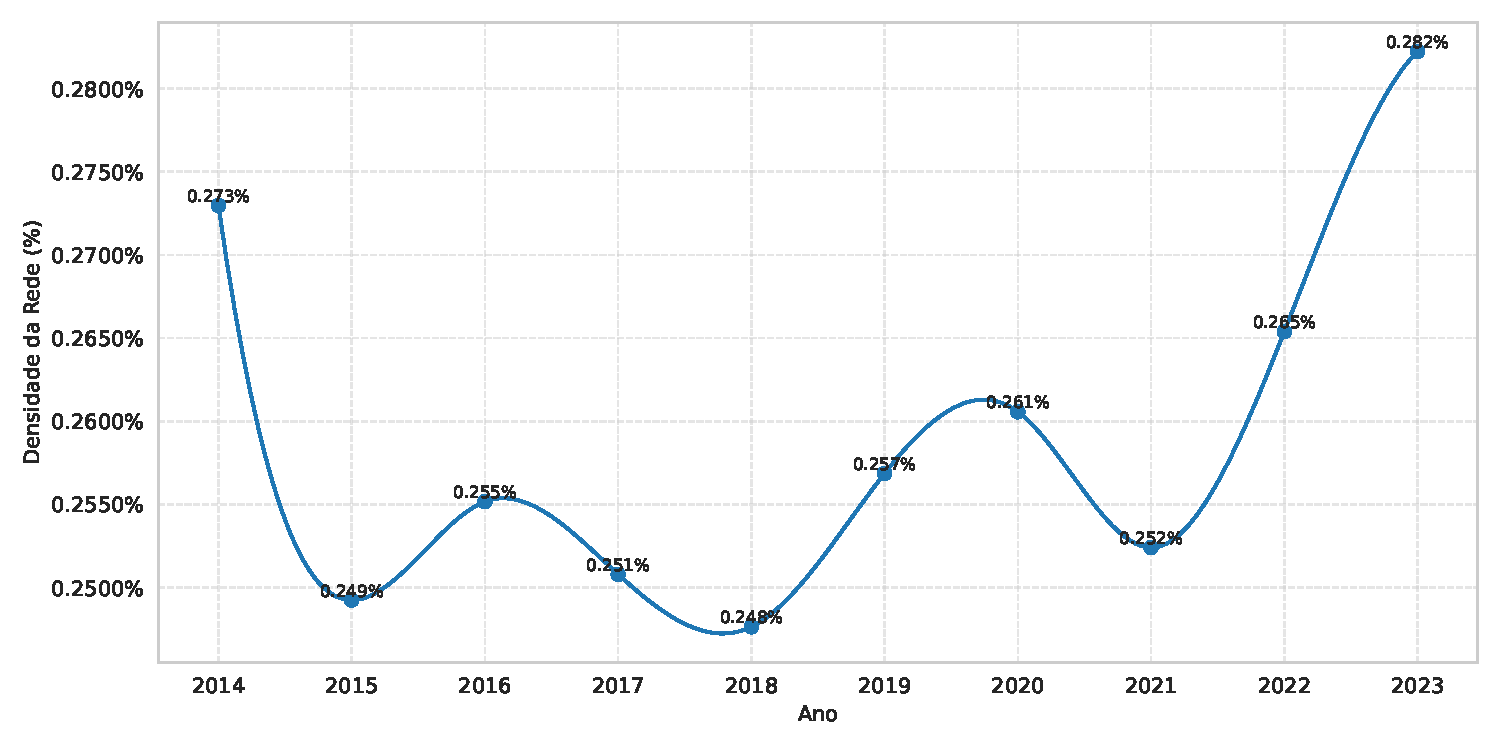
\includegraphics[width=0.9\linewidth]{figuras/density_network.pdf}
    \caption{Densidade rede 2014 a 2023}
    \label{fig:densidade}
\end{figure}

Tabel \ref{tab:densidade} apresenta kona ba porsentu densidade kada tinan husi 2014 a 2023.

\begin{table}[!ht]
    \centering
    \begin{tabular}{|c|c|}
    \hline
        \textbf{Densidade }& \textbf{Tinan } \\ \hline
        0,25\% & 2014 \\ \hline
        0,25\% & 2015 \\ \hline
        %0,21\% & 2016 \\ \hline
        %0,25\% & 2017 \\ \hline
        %0,24\% & 2018 \\ \hline
        %0,26\% & 2023 \\ \hline
    \end{tabular}
    \caption{Densidade por ano}
    \label{tab:densidade}
\end{table}


\section{Análise de rede por programas}
\section{Análise de rede por institucional}
\section{Análise de rede por ano}
%----------------------------------
%Considerações finais
%----------------------------------

%----------------------------------
\chapter{Considerações finais}
%----------------------------------

\section{Conclusão}
\section{Trabalhos futuros}

%----------------------------------------------
% Bibliography
%----------------------------------------------
\cleardoublepage
\phantomsection
\addcontentsline{toc}{chapter}{Referénsia}
\bibliographystyle{plainnat}
\bibliography{bibliografia}

\end{document}